\chapter{Arhitektura i dizajn sustava}
		
		%\textbf{\textit{dio 1. revizije}}\\

		%\textit{ Potrebno je opisati stil arhitekture te identificirati: podsustave, preslikavanje na radnu platformu, spremišta podataka, mrežne protokole, globalni upravljački tok i sklopovsko-programske zahtjeve. Po točkama razraditi i popratiti odgovarajućim skicama:}
	%\begin{itemize}
	%	\item 	\textit{izbor arhitekture temeljem principa oblikovanja pokazanih na predavanjima (objasniti zašto ste baš odabrali takvu arhitekturu)}
	%	\item 	\textit{organizaciju sustava s najviše razine apstrakcije (npr. klijent-poslužitelj, baza podataka, datotečni sustav, grafičko sučelje)}
	%	\item 	\textit{organizaciju aplikacije (npr. slojevi frontend i backend, MVC arhitektura) }		
	%\end{itemize}

	Odabrani stil je arhitektura zasnovana na događajima, točnije obrazac MVC (eng. Model-View-Controller) koji je podržan u Spring razvojnom okviru korištenjem anotacija (eng. annotations).
	
	Arhitektura se može podijeliti na tri podsustava:
	\begin{itemize}
		\item Web poslužitelj
		\item Mobilna aplikacija
		\item Baza podataka
	\end{itemize}
	
	\underline{Mobilna aplikacija} je program dizajniran za izvođenje specifičnih funkcija na mobilnom uređaju (npr. pametnom telefonu, tabletu, pametnom satu, itd.). Preko mobilne aplikacije se provodi interakcija sa korisnikom i slanje zatjeva web poslužitelju.

	\underline {Web poslužitelj} je program kojem je zadaća komunikacija sa mobilnom aplikacijom i obrada poslanih zahtjeva. Komunikacija između web poslužitelja i mobilne aplikacije se odvija na World Wide Webu koristeći HTTP (Hypertext Transfer Protocol) protokol za prijenos informacija.
	
	Korišteni programski jezik za izradu poslužiteljske aplikacije je Java sa radnim okvirom (eng. framework) Spring, dok je za izradu mobilne aplikacije korišten Dart.
	
	MVC obrazac je odabran zato što olakšava nazavisan razvoj, ispitivanje i nadogradnju dijelova aplikacije različitih namjena.
	MVC obrazac se sadrži:
	\begin{itemize}
		\item\textbf{Model} - Središnja komponenta sustava. Dinamička struktura podataka aplikacije, neovisna o korisničkom sučelju. Upravlja podacima, logikom i pravilima aplikacije.
		\item\textbf{View (Pogled)} - Bilo kakav prikaz podataka, kao što su graf, dijagram i tablica. Različiti prikazi iste informacije su mogući.
		\item\textbf{Controller (Nadglednik)} - Upravlja i rukuje korisničkom interakcijom sa modelom i pogledom (eng. vIew). Šalje naloge za korištenje podataka modelu, a pogledu šalje naloge za izmjenu prikaza.
	\end{itemize}

				
		\section{Baza podataka}
			
			%\textbf{\textit{dio 1. revizije}}\\
			
		%\textit{Potrebno je opisati koju vrstu i implementaciju baze podataka ste odabrali, glavne komponente od kojih se sastoji i slično.}
		
		Koristit ćemo relacijsku bazu podataka koja svojom strukturom zadovoljava naručiteljeve zahtjeve i olakšava korištenje. Gradivna jedinka baze je relacija, odnosno tablica koja je definirana svojim imenom i skupom atributa. Zadaća baze podataka je brza i jednostavna pohrana, izmjena i dohvat podataka za daljnju obradu. Baza podataka ove aplikacije sastoji se od sljedećih entiteta:
		\begin{itemize}
			\item Korisnik %*možda dodati tablicu klijent koja ima PayPal podatke
			\item Tvrtka
			\item Narudžba
			\item Redovna usluga
			\item Dodatna usluga
			\item Format papira
			\item Vrsta papira
			\item Boja papira
			\item Sadrži dodatnu
			\item Poruka pretplate
			\item Osnovna cijena
		\end{itemize}
			\subsection{Opis tablica}
			%\usepackage{color, colortbl}
		

				%\textit{Svaku tablicu je potrebno opisati po zadanom predlošku. Lijevo se nalazi točno ime varijable u bazi podataka, u sredini se nalazi tip podataka, a desno se nalazi opis varijable. Svjetlozelenom bojom označite primarni ključ. Svjetlo plavom označite strani ključ}
				
			%	\begin{longtabu} to \textwidth {|X[6, l]|X[6, l]|X[20, l]|}
					
				%	\hline \multicolumn{3}{|c|}{\textbf{korisnik - ime tablice}}	 \\[3pt] \hline
				%	\endfirsthead
					
					%\hline \multicolumn{3}{|c|}{\textbf{korisnik - ime tablice}}	 \\[3pt] \hline
				%	\endhead
					
				%	\hline 
				%	\endlastfoot
					
				%	\cellcolor{LightGreen}IDKorisnik & INT	&  	Lorem ipsum dolor sit amet, consectetur adipiscing elit, sed do eiusmod tempor incididunt ut labore et dolore magna aliqua. Ut enim ad minim veniam 	\\ \hline
				%	korisnickoIme	& VARCHAR &   	\\ \hline 
				%	email & VARCHAR &   \\ \hline 
				%	ime & VARCHAR	&  		\\ \hline 
				%	\cellcolor{LightBlue} primjer	& VARCHAR &   	\\ \hline 
					
					
			%	\end{longtabu}
				
				\definecolor{Celadon}{RGB}{0.67, 0.88, 0.69} %lijepa zelena
				\definecolor{grannysmithapple}{RGB}{0.66, 0.89, 0.63}  %lijepa zelena
				\definecolor{babyblueeyes}{RGB}{0.63, 0.79, 0.95}  %lijepa plava
				\definecolor{beaublue}{RGB}{0.74, 0.83, 0.9} %lijepa plava
				\definecolor{blizzardblue}{RGB}{0.67, 0.9, 0.93} %lijepa plava
				\definecolor{columbiablue}{RGB}{0.61, 0.87, 1.0} %lijepa plava
				
				
				\definecolor{Celadonm}{HTML}{ACE1AF} %lijepa zelena
				
				\textit{Podebljani atributi su primarni ključevi, dok su podcrtani vanjski ključevi.}
				\\
				
				
				\textbf{Korisnik}\newline  Ovaj entitet sadržava važne informacije o korisniku aplikacije. Sadrži atribute: korisnik\_id, email, lozinka, ime, prezime, razina\_korisnika i tvrtka\_id. Ovaj entitet je u vezi 1:0..1 s entitetom tvrtka preko atributa tvrtka\_id tvrtke, u vezi One-to-Many s entitetom narudžba preko atributa korisnik\_id korisnika i u vezi One-to-Many s entitetom dodatna\_usluga preko atributa korisnik\_id korisnika.
				\begin{longtabu} to \textwidth {|X[8, l]|X[6, l]|X[20, l]|}
					
					\hline \multicolumn{3}{|c|}{\textbf{korisnik}}	 \\[3pt]
					\hline
					\endfirsthead
					
					\hline \multicolumn{3}{|c|}{\textbf{korisnik}}	 \\[3pt]
					\hline
					\endhead
					
					\hline 
					\endlastfoot
					
					\cellcolor{LightGreen}
					\textbf{korisnik\_id}  & SERIAL  & jedinstveni identifikator korisnika\\ \hline
					email	  	 	  & VARCHAR & email koji se koristi pri prijavi	\\ \hline 
					lozinka		 	  & VARCHAR & lozinka koje se koristi i s kojom se uspoređuje pri prijavi \\ \hline 
					ime			 	  & VARCHAR & ime korisnika 						\\ \hline
					prezime		 	  & VARCHAR & prezime korisnika \\ \hline
					razina\_korisnika & INT		& razina korisnika \\
									  &			& 0 - privatni		\\
									  &			& 1 - poslovni		\\
									  &			& 2 - admin		\\ \hline
					\cellcolor{LightBlue}
					\underline{tvrtka\_id}  & INT 	   & id korisnikove tvrtke ako postoji, NULL inače
					
				\end{longtabu}
				
				\textbf{Tvrtka}\newline Ovaj entitet sadrži informacije o tvrtci za poslovne korisnike. Sadrži atribute: tvrtka\_id, tvrtka\_oib, broj\_telefona i korisnik\_id. Ovaj entitet je u vezi One-to-One sa entitetom korisnik preko korisnik\_id korisnika, te 0..1:1 sa entitetom korisnik preko tvrka\_id tvrtke.
				\begin{longtabu} to \textwidth {|X[6, l]|X[6, l]|X[20, l]|}
					
					\hline \multicolumn{3}{|c|}{\textbf{tvrtka}}	 \\[3pt] \hline
					\endfirsthead
					
					\hline \multicolumn{3}{|c|}{\textbf{tvrtka}}	 \\[3pt] \hline
					\endhead
					
					\hline 
					\endlastfoot
					
					\cellcolor{LightGreen}
					\textbf{tvrtka\_id}	& SERIAL  &		jedinstveni identifikator tvrtke	\\ \hline
					tvrtka\_oib		& VARCHAR &		OIB tvrtke							\\ \hline
					ime\_tvrtke		& VARCHAR &  	ime tvrtke							\\ \hline
					broj\_telefona	& VARCHAR &   	broj telefona kontakt osobe tvrtke	\\ \hline 
					\cellcolor{LightBlue}
					\underline{korisnik\_id} 	& INT	  &  	korisnički id tvrtke			 	\\ \hline
					
				\end{longtabu}
				
				\textbf{Narudžba}\newline  Ovaj entitet opisuje osnovne informacije o narudžbi korisnika. Sadrži atribute: narudzba\_id, korisnik\_id, cijena i datum. Ovaj entitet je u vezi Many-to-One s entitetom korisnik preko atributa korisnik\_id korisnika, u vezi One-to-Many s entitetom sadrziDodatnu preko atributa narudzba\_id i korisnik\_id narudzbe, u vezi One-to-Many s entitetom redovna\_usluga preko atributa narudzba\_id i korisnik\_id narudzbe i u vezi One-to-Many s entitetom porukaPretplate preko atributa narudzba\_id i korisnik\_id narudzbe.
				\begin{longtabu} to \textwidth {|X[8, l]|X[6, l]|X[20, l]|}
					
					\hline \multicolumn{3}{|c|}{\textbf{narudzba}}	 \\[3pt] \hline
					\endfirsthead
					
					\hline \multicolumn{3}{|c|}{\textbf{narudzba}}	 \\[3pt] \hline
					\endhead
					
					\hline 
					\endlastfoot
					
					\cellcolor{LightGreen}
					\textbf{narudzba\_id} & SERIAL	& jedinstveni identifikator narudžbe\\ \hline
					\cellcolor{LightBlue}
					\textbf{\underline{korisnik\_id}}  & INT &  jedinstveni identifikator korisnika naručitelja 	\\ \hline
					cijena 			& NUMERIC & cijena narudžbe					   	\\ \hline  
					datum 			& TIMESTAMP	& datum i vrijeme provedbe narudžbe	\\ \hline 
					
				\end{longtabu}
				
				\textbf{Dodatna usluga}\newline  Ovaj entitet opisuje sve informacije o dodatnoj usluzi za pojedinog korisnika. Sadrži atribute: dodatna\_usluga\_id, korisnik\_id, dodatna\_naziv, dodatna\_opis, cijena, kontakt\_ime, kontakt\_broj, kontakt\_email, potvrdena i pretplata. Entitet je u vezi Many-to-One s entitetom korisnik preko atributa korisnik\_id korisnika i u vezi One-to-Many s entitetom sadrziDodatnu preko atributa dodatna\_usluga\_id i korisnik\_id dodatne usluge.
				\begin{longtabu} to \textwidth {|X[10, l]|X[6, l]|X[20, l]|}
					
					\hline \multicolumn{3}{|c|}{\textbf{dodatna\_usluga}}	 \\[3pt] \hline
					\endfirsthead
					
					\hline \multicolumn{3}{|c|}{\textbf{dodatna\_usluga}}	 \\[3pt] \hline
					\endhead
					
					\hline 
					\endlastfoot
					
					\cellcolor{LightGreen}
					\textbf{dodatna\_usluga\_id} & SERIAL & jedinstveni identifikator dodatne usluge\\ \hline
					\cellcolor{LightBlue}
					\textbf{\underline{korisnik\_id}}	& INT & jedinstveni identifikator poslovnog korisnika kojem 											je usluga dodijeljena				\\ \hline 
					dodatna\_naziv	& VARCHAR & kratki naziv dodatne usluge		  						\\ \hline 
					dodatna\_opis	& VARCHAR & opis dodatne usluge										\\ \hline 
					cijena 			& NUMERIC & cijena dodatne usluge			   						\\ \hline
					kontakt\_ime 	& VARCHAR & ime kontakt osobe kompanije 							\\ \hline 
					kontakt\_broj 	& VARCHAR & broj kontakt osobe kompanije							\\ \hline 
					kontakt\_email	& VARCHAR & email kontakt osobe kompanije							\\ \hline
					potvrdena		& BOOLEAN & označava je li zahtjev potvrđen ili nije,				\\
					&		  &	ako je true onda je prihvaćen,							\\
					&		  &	ako je false onda administrator još nije donio odluku.	\\
					&		  & U slučaju da je odbijen onda entitet uklanja iz tablice 	\\ \hline
					pretplata		& BOOLEAN & označava je li narudžba mjesečna pretplata				\\ \hline
					
				\end{longtabu}
				
				\textbf{Sadrži dodatnu}\newline Entitet sadrziDodatnu sadrži informaciju koju/koje dodatne usluge sadrži narudžba. Sadrži atribute: narudzba\_id, korisnik\_id, dodatna\_usluga\_id i pretplata. Entitet sadrži vezu Many-to-One s entitetom narudzba preko atributa narudzba\_id i korisnik\_id narudžbe i vezu Many-to-One s entitetom dodatna\_usluga preko atributa dodatna\_usluga\_id i korisnik\_id dodatne usluge.
				\begin{longtabu} to \textwidth {|X[11, l]|X[6, l]|X[20, l]|}
					
					\hline \multicolumn{3}{|c|}{\textbf{sadrziDodatnu}}	 \\[3pt] \hline
					\endfirsthead
					
					\hline \multicolumn{3}{|c|}{\textbf{sadrziDodatnu}}	 \\[3pt] \hline
					\endhead
					
					\hline 
					\endlastfoot
					
					\cellcolor{LightBlue}
					\textbf{\underline{narudzba\_id}} & INT & jedinstveni identifikator narudžbe					\\ \hline
					\cellcolor{LightBlue}
					\textbf{\underline{korisnik\_id}}  & INT &  jedinstveni identifikator korisnika naručitelja 	\\ \hline
					\cellcolor{LightBlue}
					\textbf{\underline{dodatna\_usluga\_id}}		& INT & jedinstveni identifikator dodatne usluge			\\ \hline
					\cellcolor{LightBlue}
					pretplata	& BOOLEAN & označava je li narudžba mjesečna pretplata \\ \hline
				\end{longtabu}
				
				\textbf{Redovna usluga}\newline  Ovaj entitet opisuje redovnu uslugu korisnika. Sadrži entitete: narudzba\_id, korisnik\_id, visina, sirina, boja, tezina, vodeni\_zig, pretplata, format\_id, vrsta\_id i boja\_id. Entitet je u vezi Many-to-One s entitetom narudza preko atributa narudzba\_id i korisnik\_id narudžbe, u vezi Many-to-One sa format\_papira preko atributa format\_id formata papira, u vezi Many-to-One sa vrsta\_papira preko atributa vrsta\_id vrste papira, u vezi Many-to-One sa boja\_papira preko atributa boja\_id boje papira,
				\begin{longtabu} to \textwidth {|X[8, l]|X[6, l]|X[20, l]|}
					
					\hline \multicolumn{3}{|c|}{\textbf{redovna\_usluga}}	 \\[3pt] \hline
					\endfirsthead
					
					\hline \multicolumn{3}{|c|}{\textbf{redovna\_usluga}}	 \\[3pt] \hline
					\endhead
					
					\hline 
					\endlastfoot
					
					\cellcolor{LightBlue}
					\underline{narudzba\_id} 	& SERIAL  & jedinstveni identifikator narudzbe						\\ \hline
					\cellcolor{LightBlue}
					\underline{korisnik\_id}	& INT 	  & jedinstveni identifikator korisnika naručitelja			\\ \hline 
					visina			& INT	  & visina papira u mm		  								\\ \hline 
					sirina			& INT	  & širina papira u mm										\\ \hline 
					boja 			& VARCHAR & heksadecimalni zapis boje papira   						\\ \hline
					tezina		 	& VARCHAR & težina papira u gsm			 							\\ \hline
					vodeni\_zig		& BLOB	  & slika vodenog žiga										\\ \hline
					pretplata		& BOOLEAN & označava je li narudžba mjesečna pretplata				\\ \hline
					\cellcolor{LightBlue}
					\underline{format\_id} 		& INT 	  & jedinstveni identifikator formata papira,				\\
					&		  &	0 je rezerviran za nekonvencionalne formate 			\\ \hline
					\cellcolor{LightBlue}
					\underline{vrsta\_id} 		& INT	  & jedinstveni identifikator vrste papira					\\ \hline
					\cellcolor{LightBlue}
					\underline{boja\_id} 		& INT	  & jedinstveni identifikator boje papira					\\
					&		  &	0 je rezerviran za proizvoljne boje						\\ \hline  
					
					
					
				\end{longtabu}
				
				\textbf{Format papira}\newline	Ovaj entitet sadrži sve informacije o formatu papira. Sadrži atribute format\_id, format\_ime, visina, sirina i koeficijent\_cijena. Entitet je u vezi One-to-Many s entitetom redovna\_usluga preko atributa format\_id formata papira.
				\begin{longtabu} to \textwidth {|X[8, l]|X[6, l]|X[20, l]|}
					
					\hline \multicolumn{3}{|c|}{\textbf{format\_papira}}	 \\[3pt] \hline
					\endfirsthead
					
					\hline \multicolumn{3}{|c|}{\textbf{format\_papira}}	 \\[3pt] \hline
					\endhead
					
					\hline 
					\endlastfoot
					
					\cellcolor{LightGreen}
					\textbf{format\_id} 			& SERIAL  & jedinstveni identifikator formata papira,			\\
					&		  &	0 je rezerviran za nekonvencionalne formate 		\\ \hline
					format\_ime			& VARCHAR & ime formata papira									\\ \hline 
					visina 				& INT	  & visina formata papira u mm							\\ \hline 
					širina 				& INT	  & širina formata papira u mm							\\ \hline 
					koeficijent\_cijena	& NUMERIC & cijena narudžbe				   						\\ \hline 
					
				\end{longtabu}
				
				\textbf{Vrste papira}\newline	Ovaj entitet sadrži sve informacije o vrsti papira. Sadrži atribute vrsta\_id, vrsta\_ime i koeficijent\_cijena. Entitet je u vezi One-to-Many s entitetom redovna\_usluga preko atributa vrsta\_id vrste papira.
				\begin{longtabu} to \textwidth {|X[8, l]|X[6, l]|X[20, l]|}
					
					\hline \multicolumn{3}{|c|}{\textbf{vrste\_papira}}	 \\[3pt] \hline
					\endfirsthead
					
					\hline \multicolumn{3}{|c|}{\textbf{vrste\_papira}}	 \\[3pt] \hline
					\endhead
					
					\hline 
					\endlastfoot
					
					\cellcolor{LightGreen}
					\textbf{vrsta\_id} 			& SERIAL  & jedinstveni identifikator vrste papira				\\ \hline 
					vrsta\_ime 			& VARCHAR & ime vrste papira									\\ \hline 
					koeficijent\_cijena	& NUMERIC & cijena narudžbe				   						\\ \hline  
					
				\end{longtabu}
				
				\textbf{Boja papira}\newline	Ovaj entitet sadrži sve informacije o boji papira. Sadrži atribute boja\_id, boja\_ime, hexcode i koeficijent\_cijena. Entitet je u vezi One-to-Many s entitetom redovna\_usluga preko atributa boja\_id boje papira.
				\begin{longtabu} to \textwidth {|X[8, l]|X[6, l]|X[20, l]|}
					
					\hline \multicolumn{3}{|c|}{\textbf{boja\_papira}}	 \\[3pt] \hline
					\endfirsthead
					
					\hline \multicolumn{3}{|c|}{\textbf{boja\_papira}}	 \\[3pt] \hline
					\endhead
					
					\hline 
					\endlastfoot
					
					\cellcolor{LightGreen}
					\textbf{boja\_id} 			& SERIAL  & jedinstveni identifikator boje papira				\\
					&		  &	0 je rezerviran za proizvoljne boje					\\ \hline  
					ime\_boja 			& VARCHAR & ime boje papira										\\ \hline 
					koeficijent\_cijena	& NUMERIC & cijena narudžbe				   						\\ \hline
					hexcode				& VARCHAR & heksadecimalni zapis boje papira					\\ 
					
				\end{longtabu}
			
				\textbf{Poruka pretplate}\newline	Ovaj entitet sadrži osnovne informacije o porukama pretplate. Entitet se svakih 24h treba ažurirati i dodati unos za korisnika i narudžbu sa pretplatom koja je naručena na ovaj dan u mjesecu. Nakon što je korisnik primio redak on se treba obrisati, te nepojavljivati nadalje. Narudžba\_id je vanjski ključ na narudžba\_id narudžbe, kako bi znali da se pretplate, redovne\_usluge ili dodatne\_usluge\, nalaze u nekoj narudžbi. Korisnik\_id je vanjski ključ za korisnik\_id korisnika i preko njega jednostavno znamo kojemu korisniku treba biti prikazana poruka.
				Sadrži atribute: id, narudžba\_id i korisnik\_id.
				Entitet je u vezi Many-to-One s entitetom narudzba preko atributa narudzba\_id i korisnik\_id narudžbe.
				\begin{longtabu} to \textwidth {|X[8, l]|X[6, l]|X[20, l]|}
					
					\hline \multicolumn{3}{|c|}{\textbf{porukaPretplate}}	 \\[3pt] \hline
					\endfirsthead
					
					\hline \multicolumn{3}{|c|}{\textbf{porukaPretplate}}	 \\[3pt] \hline
					\endhead
					
					\hline 
					\endlastfoot
					
					\cellcolor{LightGreen}
					\textbf{id} 			& SERIAL  & jedinstveni identifikator mjesečne poruke o provedbi pretplate	\\ \hline  
					\underline{narudzba\_id} 	& INT & jedinstveni identifikator narudžbe\\ \hline 
					\underline{korisnik\_id} 	& INT & jedinstveni identifikator korisnika\\
					
				\end{longtabu}
			
				\textbf{Osnovna cijena}\newline	Ovaj entitet sadrži informaciju o osnovnoj cijeni proizvoda. Sadrži atribut: cijena. Tablica ima samo jedan unos.
				\begin{longtabu} to \textwidth {|X[8, l]|X[6, l]|X[20, l]|}
					
					\hline \multicolumn{3}{|c|}{\textbf{osnovna\_cijena}}	 \\[3pt] \hline
					\endfirsthead
					
					\hline \multicolumn{3}{|c|}{\textbf{osnovna\_cijena}}	 \\[3pt] \hline
					\endhead
					
					\hline 
					\endlastfoot
					
					\cellcolor{LightGreen}
					cijena 	& NUMERIC & osnovna cijena proizvoda koja se množi sa koeficijentima cijena kako bi se dobila cijena neke redovne usluge\\
					
				\end{longtabu}
			\newpage
			
			\subsection{Dijagram baze podataka}
			%	\textit{ U ovom potpoglavlju potrebno je umetnuti dijagram baze podataka. Primarni i strani ključevi moraju biti označeni, a tablice povezane. Bazu podataka je potrebno normalizirati. Podsjetite se kolegija "Baze podataka".}
			
			\begin{figure}[H]
				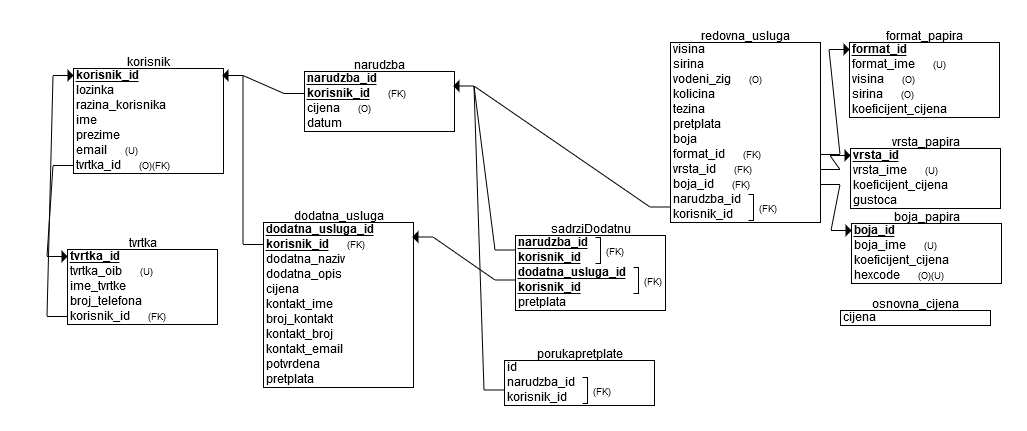
\includegraphics[scale=0.5]{dijagrami/dijagram_baze_podataka.PNG} 
				\centering
				\caption{ER dijagram baze podataka}
				\label{fig:dij_bp1}%label mora biti drugaciji za svaku sliku
			\end{figure}
			
		
		\newpage	
		\section{Dijagram razreda}
		
		%	\textit{Potrebno je priložiti dijagram razreda s pripadajućim opisom. Zbog preglednosti je moguće dijagram razlomiti na više njih, ali moraju biti grupirani prema sličnim razinama apstrakcije i srodnim funkcionalnostima.}\\
			
			%\textbf{\textit{dio 1. revizije}}\\
			
			%\textit{Prilikom prve predaje projekta, potrebno je priložiti potpuno razrađen dijagram razreda vezan uz \textbf{generičku funkcionalnost} sustava. Ostale funkcionalnosti trebaju biti idejno razrađene u dijagramu sa sljedećim komponentama: nazivi razreda, nazivi metoda i vrste pristupa metodama (npr. javni, zaštićeni), nazivi atributa razreda, veze i odnosi između razreda.}\\
			
			%\textbf{\textit{dio 2. revizije}}\\			
			
		%	\textit{Prilikom druge predaje projekta dijagram razreda i opisi moraju odgovarati stvarnom stanju implementacije}
			
			Prikazani razredi se odnose na backend MVC arhitekturu. Dijagram razreda je podijeljen po ulogama na 3 podskupine, controlleri, servici i modeli. Controlleri primaju određene HTTP zahtjeve te pozivaju potrebne servicee koji te zahtjeve dalje obrađuju koristeći potrebne DAO-e (eng. Data Access Object) za komunikaciju sa bazom podataka. Razredi koji se manipuliraju u programu se nalaze u modelu.
			
			\begin{figure}[H]
				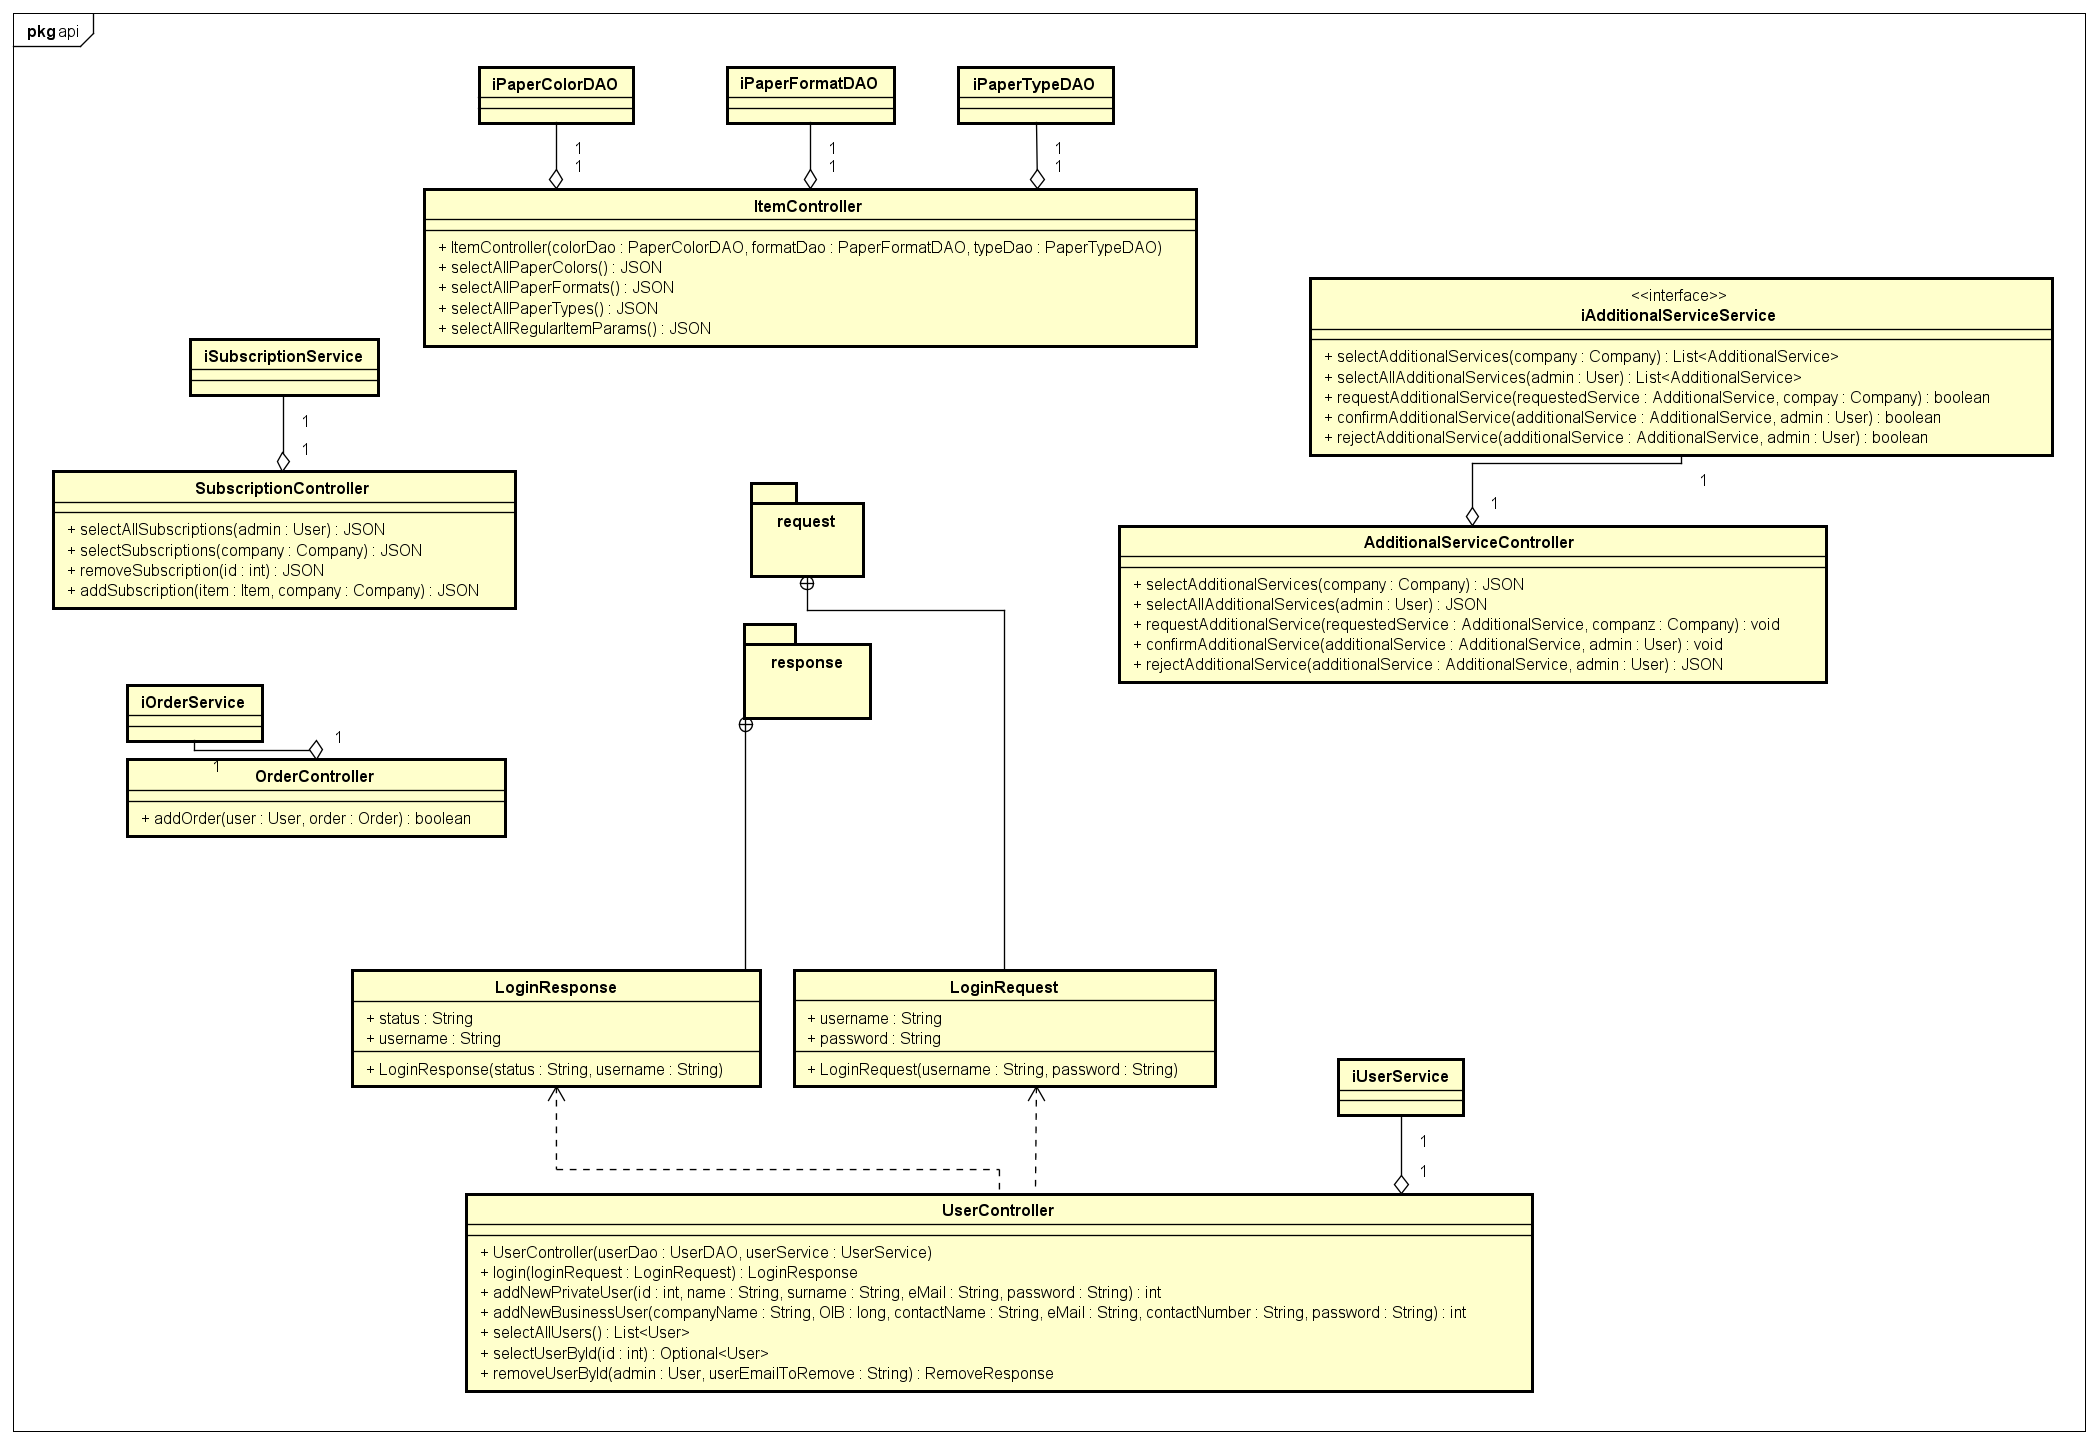
\includegraphics[scale=0.33]{dijagrami/dij_raz_cont.PNG} 
				\centering
				\caption{Dijagram razreda - controlleri}
				\label{fig:dij_raz1}%label mora biti drugaciji za svaku sliku
			\end{figure}
			
			\begin{figure}[H]
				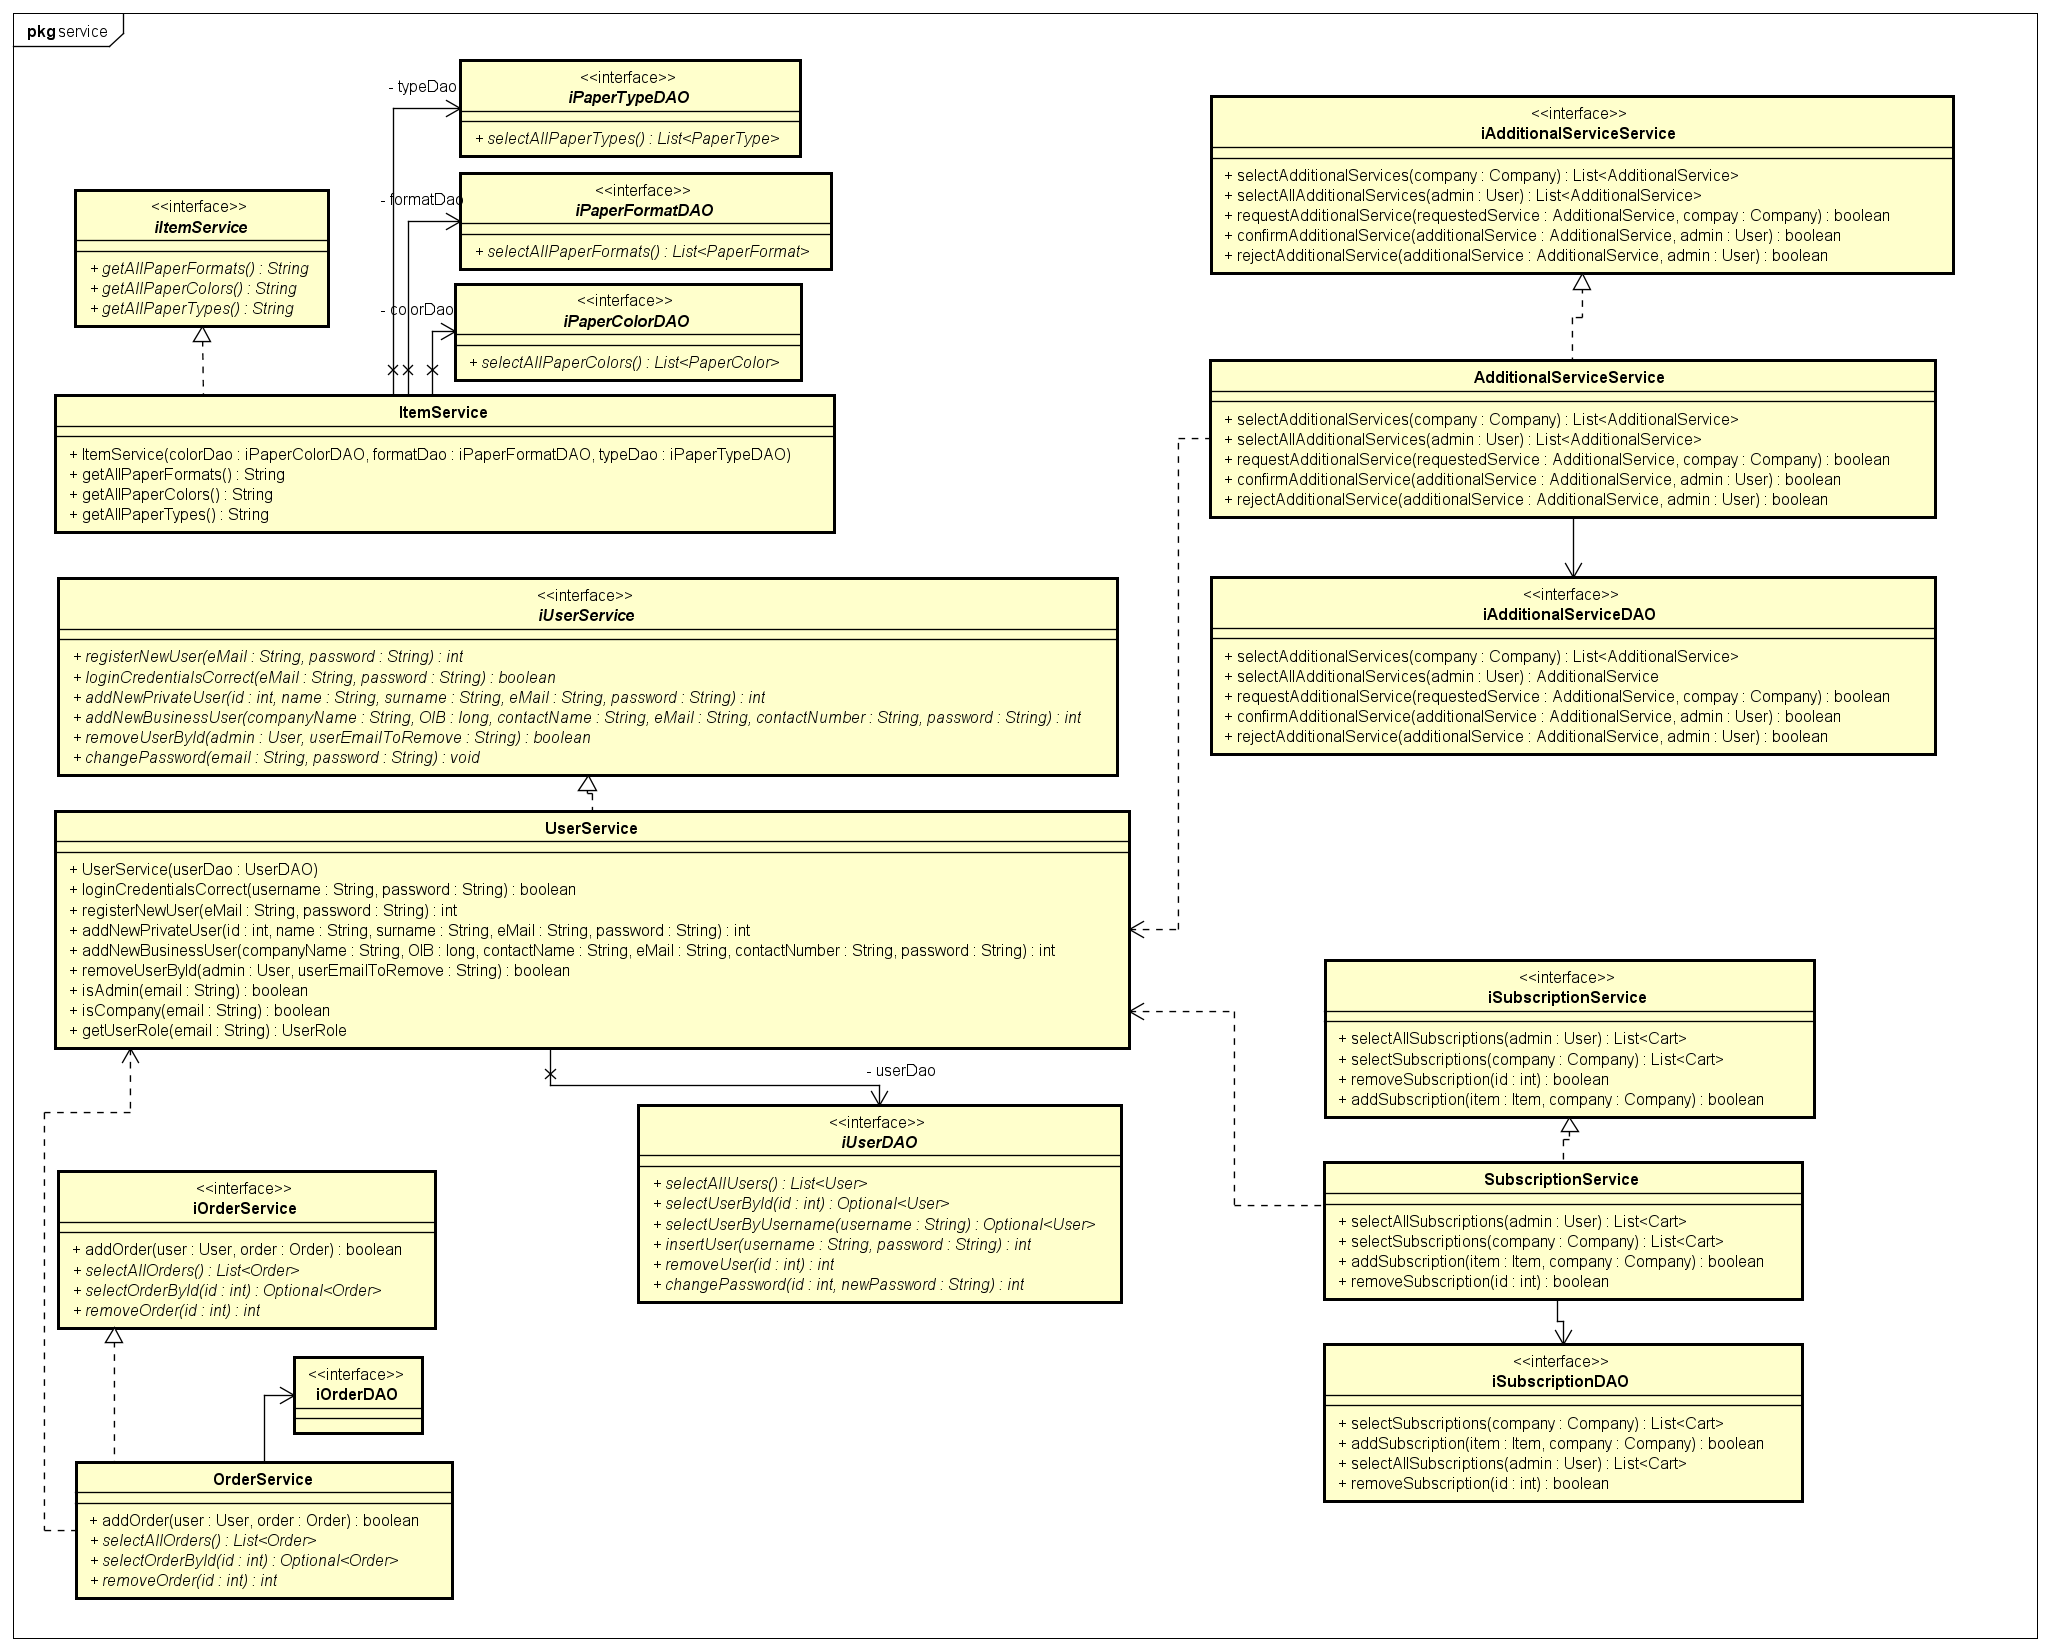
\includegraphics[scale=0.34]{dijagrami/dij_raz_serv.PNG} 
				\centering
				\caption{Dijagram razreda - servici}
				\label{fig:dij_raz2}%label mora biti drugaciji za svaku sliku
			\end{figure}
			
			\begin{figure}[H]
				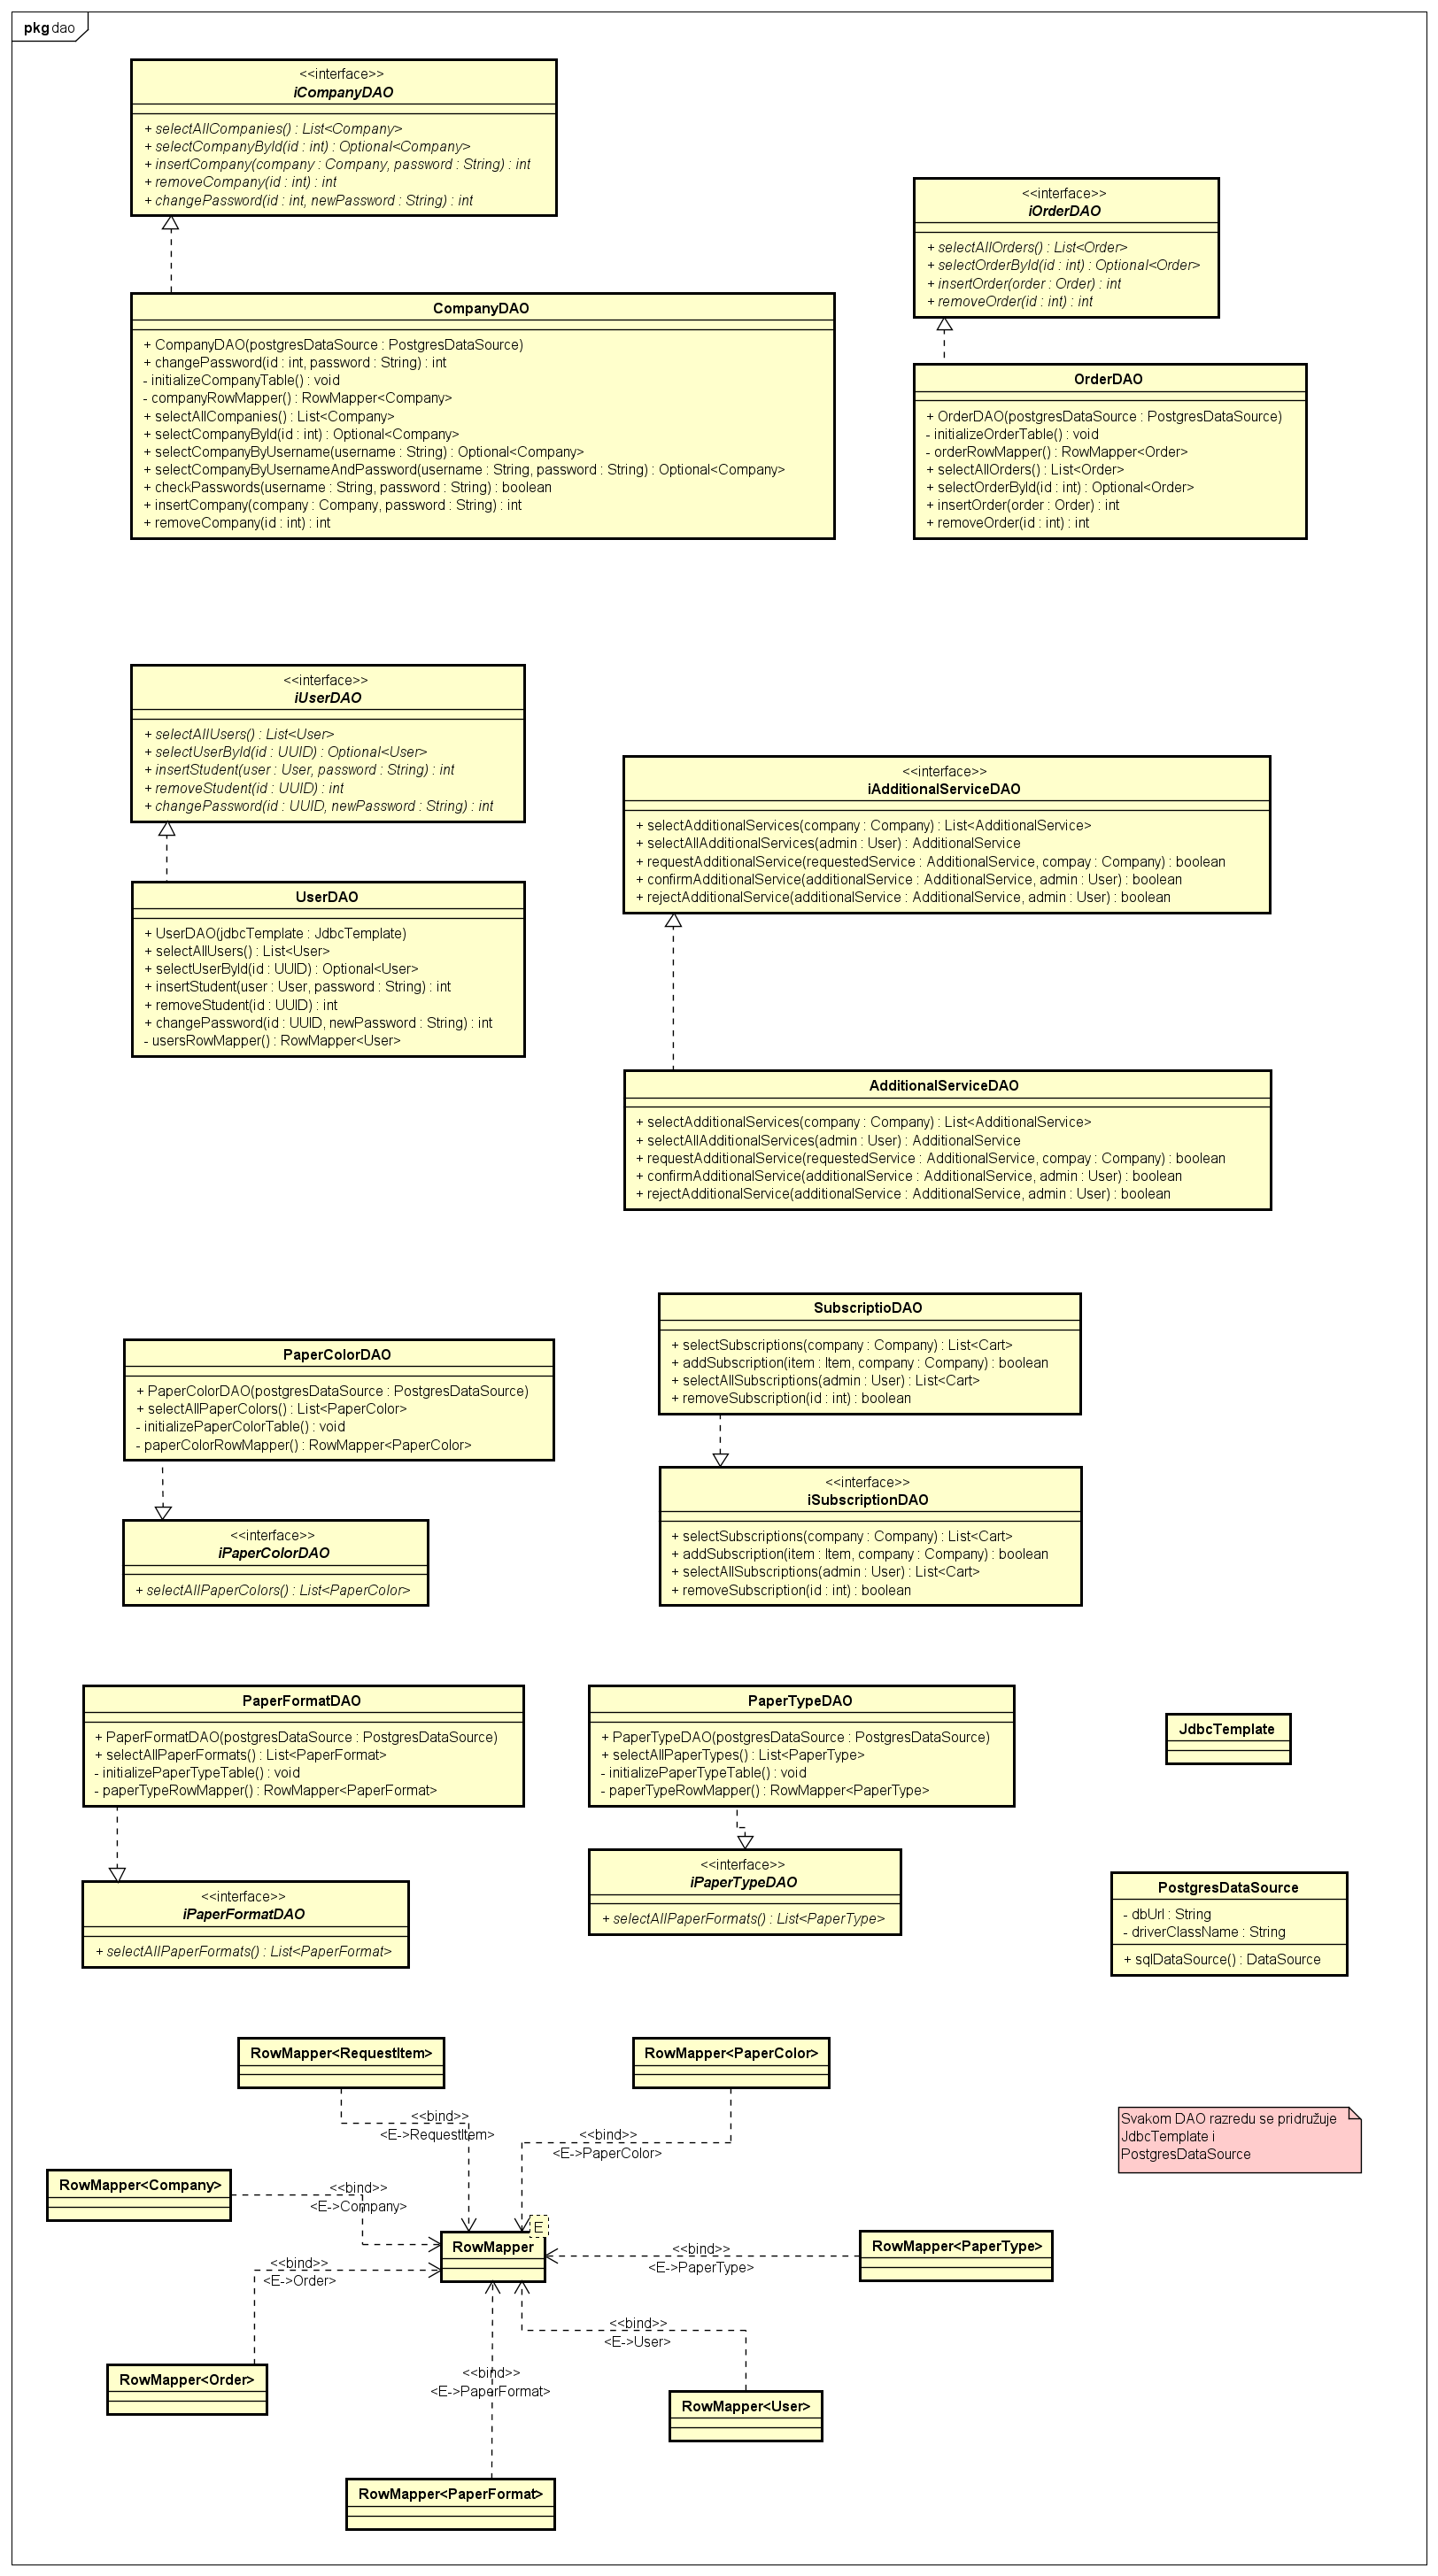
\includegraphics[scale=0.29]{dijagrami/dij_raz_dao_ureden.PNG} 
				\centering
				\caption{Dijagram razreda - DAO-i}
				\label{fig:dij_raz3}%label mora biti drugaciji za svaku sliku
			\end{figure}
		
			\begin{figure}[H]
				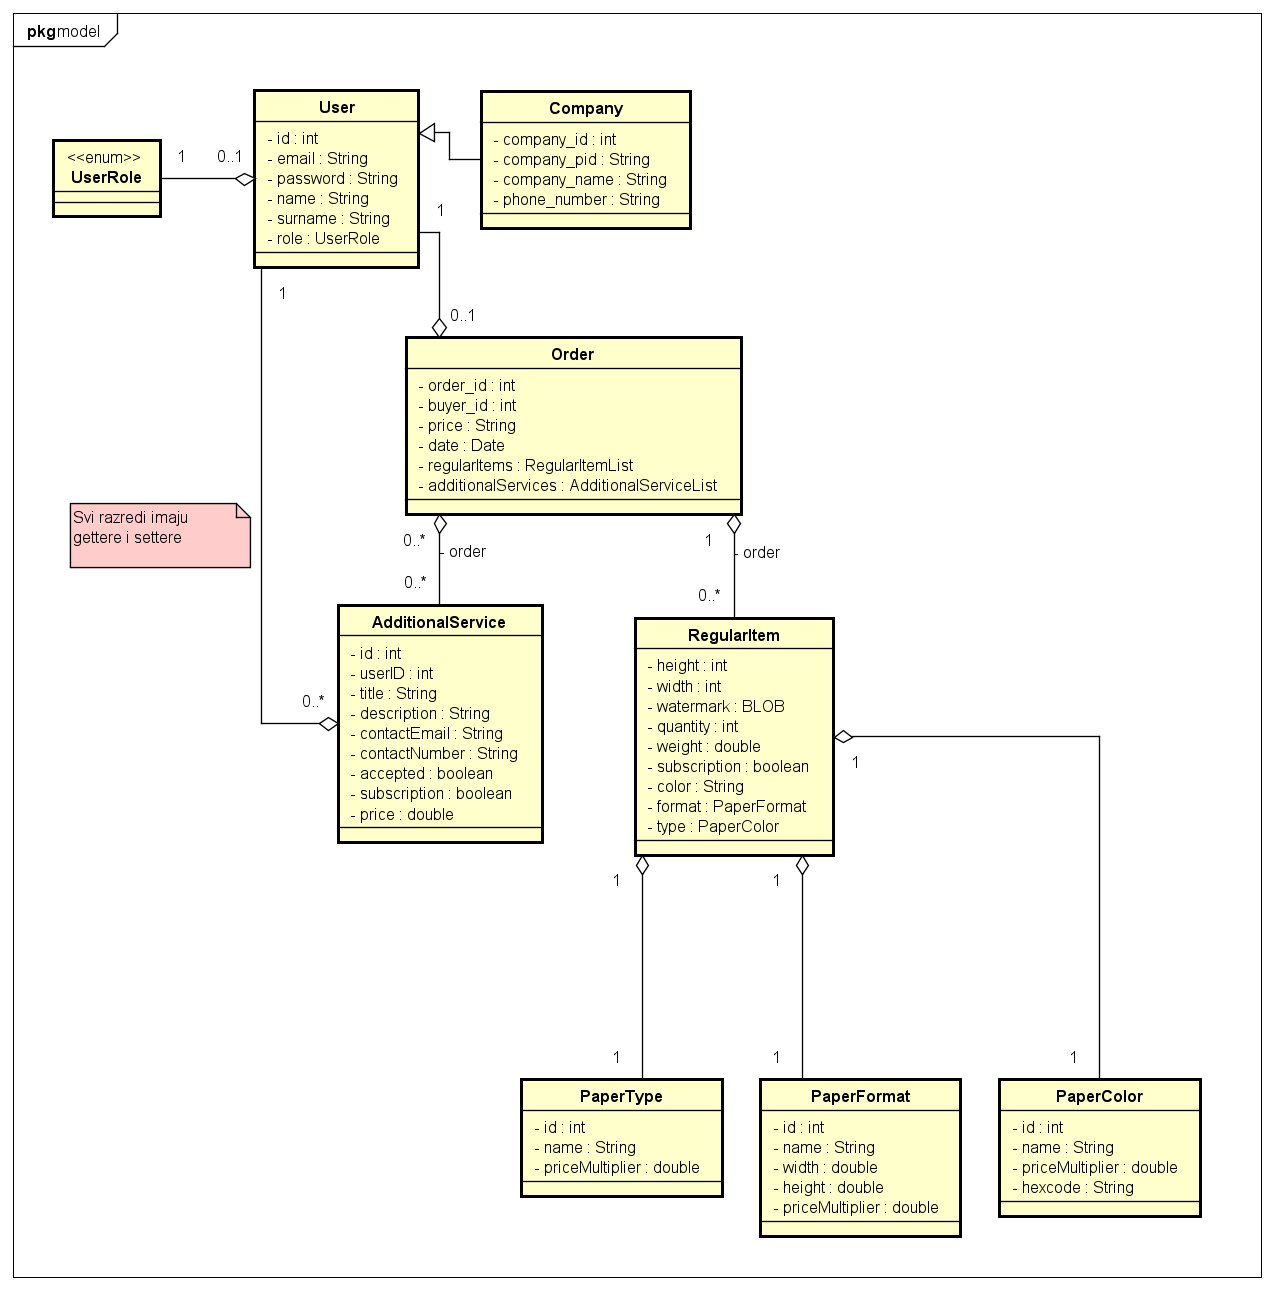
\includegraphics[scale=0.4]{dijagrami/dij_raz_model.PNG} 
				\centering
				\caption{Dijagram razreda - modeli}
				\label{fig:dij_raz4}%label mora biti drugaciji za svaku sliku
			\end{figure}
			
			\eject
		
		\section{Dijagram stanja}
			Dijagram stanja prikazuje stanja objekta te prijelaze iz jednog stanja u drugo temeljene na događajima. Na slici je prikazan dijagram stanja za poslovnog korisnika, registriranog ili ne. Nakon prijave ili registracije, klijentu se odmah prikazuje stranica "Narudžbe" na kojoj može vidjeti svoje dosadašnje narudžbe, stvoriti nove te ih dodati u košaricu. U svakom trenutku klijent se može pozicionirati u svoj "Profil", u "Zahtjeve" ili u navedene "Narudžbe" i "Košaricu". Ukoliko se pozicionira u "Zahtjeve", tamo može pregledavati status postojećih zahtjeva ili stvoriti novi zahtjev klikom na "Novi zahtjev", te iste može dodati u košaricu klikom na ikonicu košarice što ga ponovo prebacuje na "Košaricu". Ukoliko se pozicionira u "Profil", od tamo može pristupiti svojim pretplatama klikom na "Popis pretplata", gdje ih zatim može dodavati i brisati. Iz "Profila" se također može odjaviti što ga prebacuje na početnu stranicu "Prijave".
			\\
			\begin{figure}[H]
				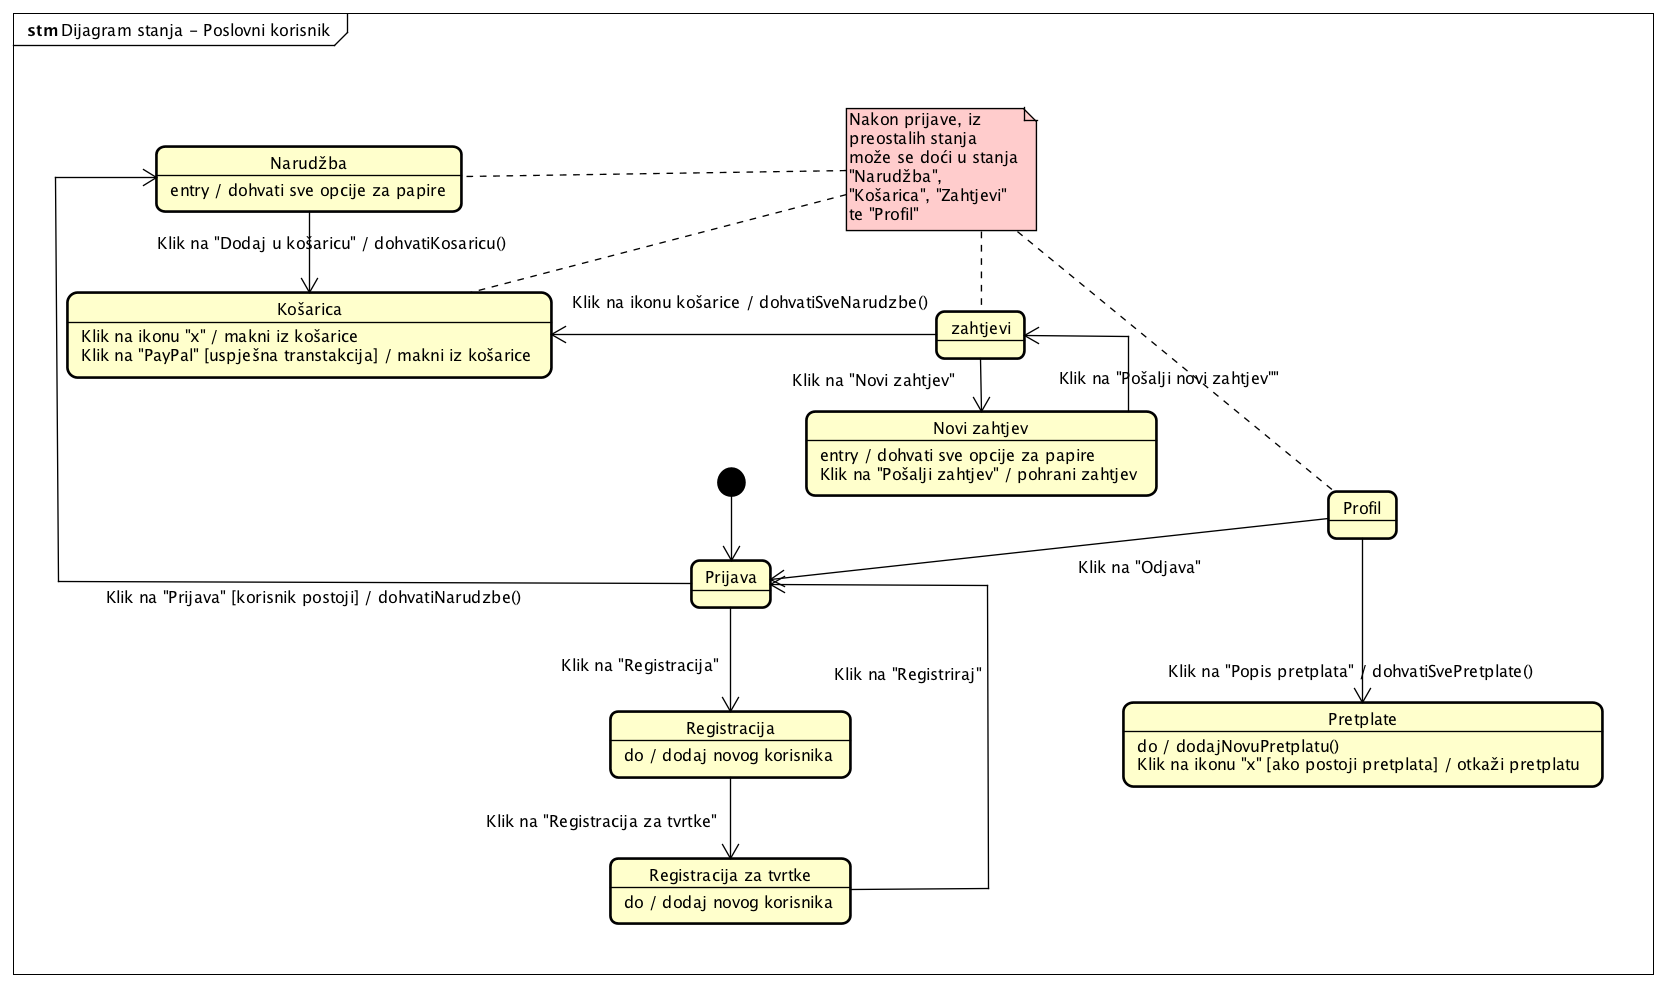
\includegraphics[scale=0.4]{dijagrami/dij_stanja.PNG} 
				\centering
				\caption{Dijagram stanja}
				\label{fig:dij_stanja}%label mora biti drugaciji za svaku sliku
			\end{figure}
			%\textbf{\textit{dio 2. revizije}}\\
			
		%	\textit{Potrebno je priložiti dijagram stanja i opisati ga. Dovoljan je jedan dijagram stanja koji prikazuje \textbf{značajan dio funkcionalnosti} sustava. Na primjer, stanja korisničkog sučelja i tijek korištenja neke ključne funkcionalnosti jesu značajan dio sustava, a registracija i prijava nisu. }
			
			
			\eject 
		
		\section{Dijagram aktivnosti}
			
			%\textbf{\textit{dio 2. revizije}}\\
			
			 
			 Dijagram aktivnosti koristi se za prikaz poslovnih procesa te upravljačkog i podatkovnog toka. On je prigodan za opis sinkronizacije i konkurentnosti, no ne i za modeliranje događajima poticanog ponašanja.
			 \\
			 Sljedeći dijagram prikazuje proces kreiranja narudžbe u slučaju privatnog korisnika. Korisnik se prijavi u sustav, odabire što želi naručiti te potom, nakon što izabere sve što mu je potrebno, odabire pregled košarice i plaća narudžbu te se ona naplaćuje.
			 \\
			 \begin{figure}[H]
			 	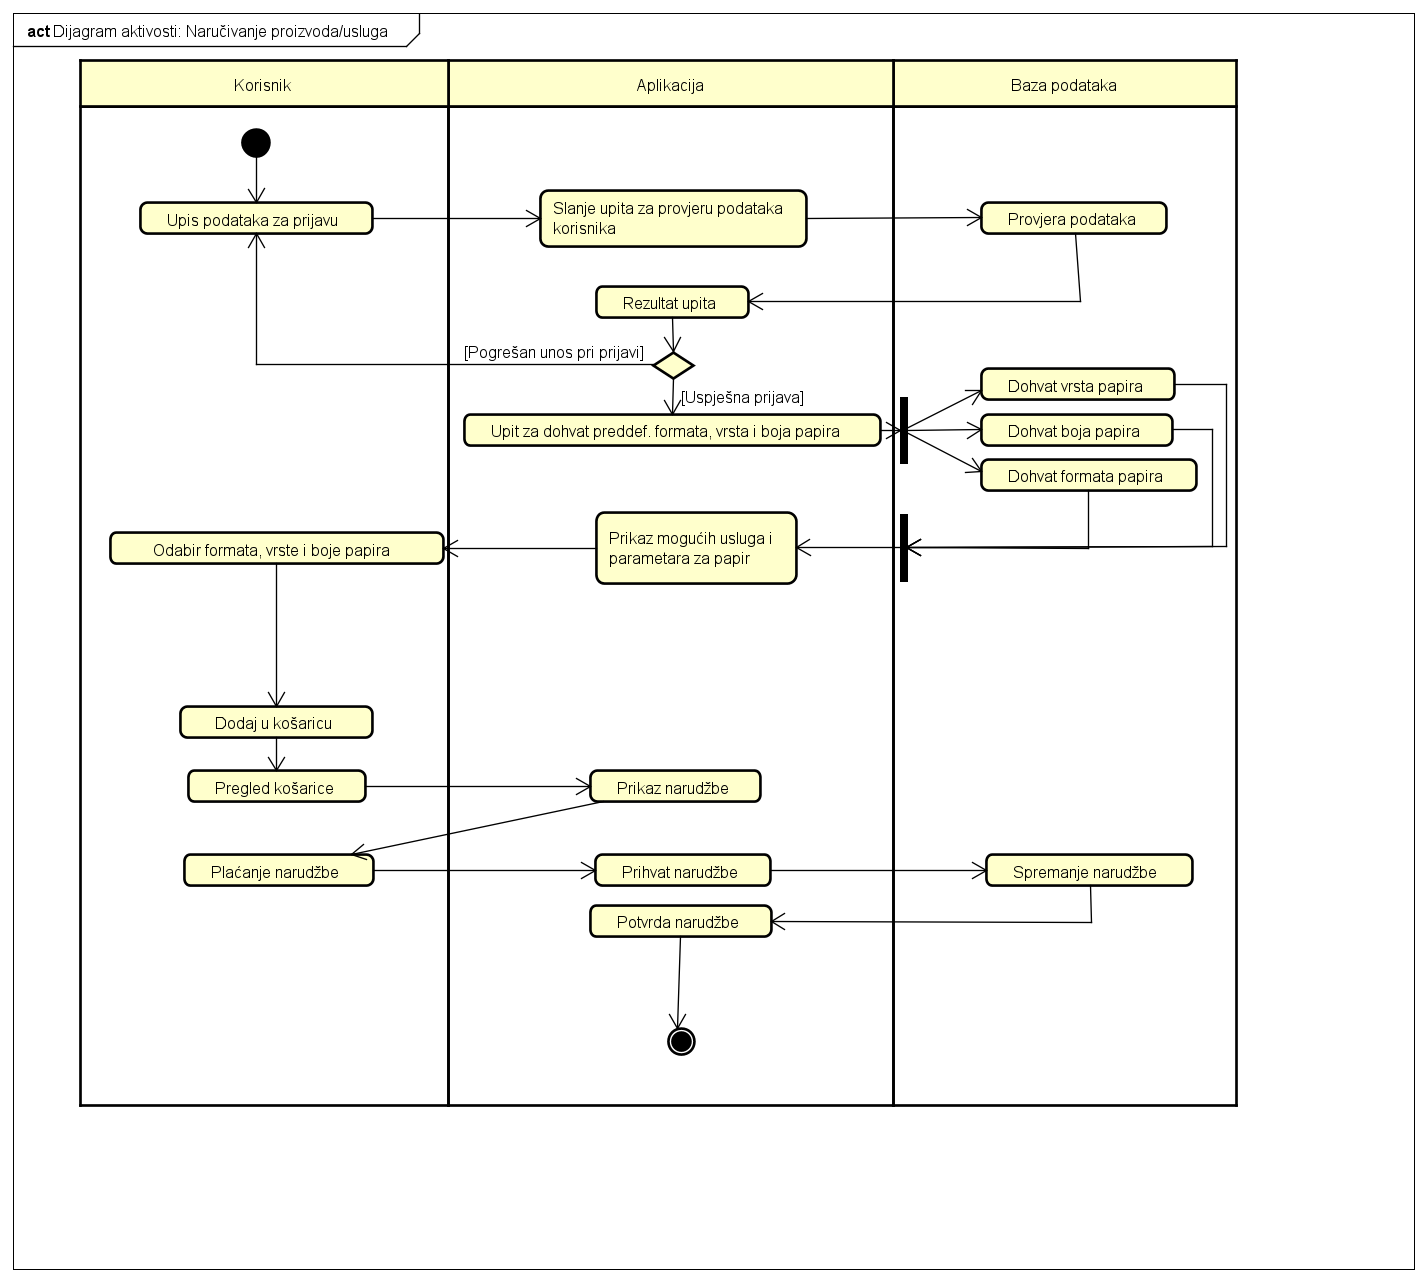
\includegraphics[scale=0.5]{dijagrami/dijagram_aktivnosti.PNG} 
			 	\centering
			 	\caption{Dijagram aktivnosti}
			 	\label{fig:dij_akt}%label mora biti drugaciji za svaku sliku
			 \end{figure}
			
			
			
			\eject
		\section{Dijagram komponenti}
			Dijagram komponenti prikazan na slici  opisuje organizaciju i međuovisnost
			komponenti, interne strukture i odnose prema okolini. Sustavu se pristupa preko sučelja. Klijent pristupa web aplikaciji koristeći web preglednik i sučelje REST API. Web aplikacija organizirana je modularno prema pravilima radnog okvira Java Spring Boota. Modul DAO je zadužen za dohvat i obradu podatka iz baze preko sučelja SQL API te povezivanje istih s Modelom predstavlja klase sustava.  Modul Service zatim te podatke obraduje na aplikaciji svojstven način, a modul Controllers je zadužen za komunikaciju HTTPS protokolom sa Klijentom.
			
			\begin{figure}[H]
				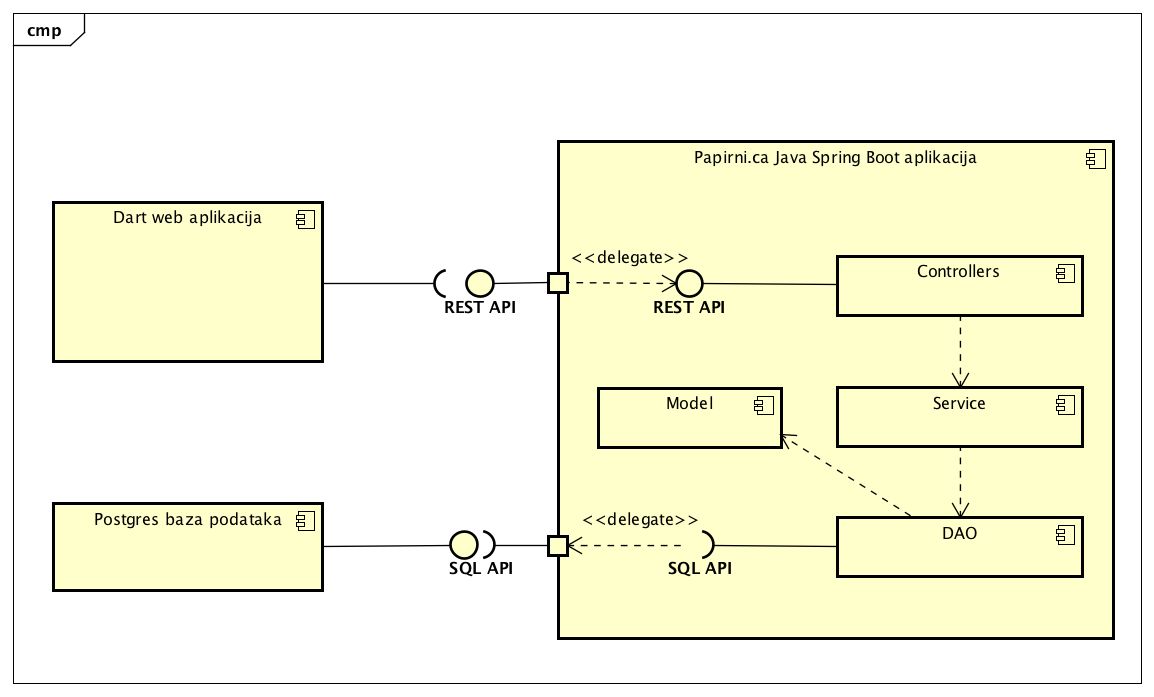
\includegraphics[scale=0.55]{dijagrami/dij_komp.PNG} 
				\centering
				\caption{Dijagram komponenti}
				\label{fig:dij_komp}%label mora biti drugaciji za svaku sliku
			\end{figure}
			%\textbf{\textit{dio 2. revizije}}\\
		
		%	 \textit{Potrebno je priložiti dijagram komponenti s pripadajućim opisom. Dijagram komponenti treba prikazivati strukturu cijele aplikacije.}